\section{String dynamics in a solenoid: the near-miss mechanism (P1 theory)}\label{sec:string}

This section derives how a uniform magnetic field thickens the quirk plane. The derivation is classical Nambu--Goto (NG)
string theory with massive point ends; it is summarised from the Stage-1 note \rep{analytic/NEAR_MISS_IMPULSE.md}
(v5.1), whose sympy checks (\rep{analytic/checks/}) and blind numerics (\rep{analytic/numerics/NUMERICS.md}) give every
step. Prior work that is used is credited at the point of use, following the novelty audit
\rep{analytic/NOVELTY_AUDIT.md}. Appendix~\ref{app:derivation} gives the full derivation step by step, with every intermediate result and the
check that verifies it; this section states the results and their status.

\subsection{Setup and observable}\label{sec:string:setup}
The ends have equal masses $\mQ$ and charges $\pm q$ (in units of $e$), the string has tension $\sigma$ and the endpoint
equations of motion are those of Kang and Luty~\cite{Kang:2008ea} plus the Lorentz force. A uniform lab field
$\mathbf B$ is, in the frame of the initial pair velocity $\boldsymbol\beta_{\rm cm}$, a uniform pair of fields
$\Estar=\gamma_{\rm cm}\boldsymbol\beta_{\rm cm}\times\mathbf B$ and $\Bstar$. The dimensionless field strengths are
\begin{equation}
  \epsB\equiv\frac{qB}{\sigma}=2.254\times10^{-4}\,\frac{B}{3.8112\tesla}\left(\frac{\keV}{\Lam}\right)^2,\qquad
  \epsp\equiv\frac{q|\Estar_\perp|}{\sigma},\qquad \kB\equiv\frac{|\Bstar_\perp|}{|\Estar_\perp|},
  \label{eq:eps}
\end{equation}
where $\perp$ refers to the initial oscillation axis $\hat n$. Without fields the exact solution is the yo-yo of
Section~\ref{sec:model:bench}: the ends pass through each other on a line, and the hits lie exactly on a plane through
the production vertex.

The observable is the plane thickness
\begin{equation}
  \Ds=\sqrt{\lambda_{\min}(T)},\qquad T_{ij}=\frac{1}{N-1}\sum_{a=1}^{N}h^a_i h^a_j ,
  \label{eq:ds}
\end{equation}
over all hits $h^a$ of both quirks on the ten Phase-2 barrel layers ($R=3.0$--$108.3\cm$), with the plane through the
primary vertex~\cite{Knapen:2017kly,Li:2020aoq}. $\DsB$ denotes $\Ds$ at truth level with the field and no material;
the vacuum value is zero.

\subsection{Torque, angular momentum and the odd-crossing miss distance}\label{sec:string:b}
The string is neutral and the magnetic forces on the two ends cancel in the relative motion, so only $\Estar$ exerts a
torque: $d\mathbf J/dt=q(\mathbf x_1-\mathbf x_2)\times\Estar$. On the yo-yo the separation reverses every half
period, $x(t+T_h)=-x(t)$, so $\mathbf J$ grows during one half period and is returned during the next: it is zero at
even crossings and maximal at odd ones. At a crossing the string has zero length and $\mathbf J=b\,p^*$, so the ends
miss each other at odd crossings by~(\rep{NEAR_MISS} \S3.2; derived; checked to $10^{-4}$ with the causal solver and to $\le10^{-3}$ with two solvers)
\begin{equation}
  \bodd = 2\,\epsp\,\lzero\left[\gst-\frac{\operatorname{asinh}(\gst\bst)}{\gst\bst}\right],
  \label{eq:bodd}
\end{equation}
and meet head-on at even ones. In the non-relativistic limit Eq.~\eqref{eq:bodd} becomes
$\tfrac43 q|\Estar_\perp|\mQ\beta^{*2}/\sigma^2$, and it vanishes for $\Estar\to0$, as it must. For $\mQ=500\GeV$ at
$3.8\tesla$ its median is $\approx3.5\um\,(\keV/\Lam)^4$. The $\mQ B/\Lam^4$ scale of the field-induced separation
``after one oscillation'' was first estimated by Kang and Luty~\cite[Eq.~(5.64)]{Kang:2008ea}; Li et al.'s $d_E$ has
the same scaling~\cite[Eq.~(V.8)]{Li:2020aoq}. The thickness formula $d\approx1.16\um\,(\mQ/100\GeV)(\keV/\Lam)^4(B/\mathrm
T)$ of Ref.~\cite[Eq.~(III.12)]{Li:2019wce} also has this scaling: it measures the miss distance, not the accumulated
plane-fit thickness, which scales differently (Section~\ref{sec:string:law}).

\subsection{Why first-order perturbation theory fails at odd crossings}\label{sec:string:breakdown}
Linearising in the field, the transverse relative coordinate $z$ of a straight string obeys
$\mu\ddot z=-\sigma z/|x(t)|+q|\Estar_\perp|$ with $\mu=\mQ/2$. Near a crossing $|x|\simeq2v|s|$ ($s$ the time from the
crossing, $v=\bst$), so $\sigma/|x|\propto1/|s|$ and the impulse $\int\sigma z/|x|\,ds$ diverges logarithmically unless
$z=0$ at the crossing. At production and at even crossings $z=0$ and the linear theory is exact (the response before
the first crossing is linear to $10^{-4}$ in the numerics); at odd crossings $z=\bodd\neq0$ and the impulse is
$\propto b\ln(1/b)$. First-order perturbation theory therefore fails at every odd crossing and only there; Li et al.\
noted that the first-order solution fails on the approach to the crossing~\cite[App.~A]{Li:2020aoq}.

The exact NG solution in the intermediate region $\bodd\ll|x|\ll\lzero$ resolves the divergence. There the string piece is
light and slaved to the ends; for ends at transverse offsets $\pm b/2$ moving at $x=\pm vs$ the static-gauge solution of
$y_{tt}=y_{xx}$ is (\rep{NEAR_MISS} \S3.4)
\begin{equation}
  y(s,x)=\frac b2\,\frac{\operatorname{artanh}(x/s)}{\operatorname{artanh}v},\qquad
  F_\perp=\mp\frac{\sigma b}{2|s|\operatorname{artanh}v},
  \label{eq:intermediate}
\end{equation}
which reduces to the straight-string pull $\sigma b/(2v|s|)$ for $v\to0$; the factor $1/\operatorname{artanh}v$ instead
of $1/v$ is the retardation effect. Integrated over the intermediate region on both sides, the relative transverse
momentum changes by $(\sigma b/\operatorname{artanh}\bst)[\ln(\lmax/b)+O(1)]$. Because the string carries
no momentum at the crossing, a transverse momentum $\Delta p_\perp$ acquired there rotates all later motion rigidly by
$\Delta p_\perp/p^*$ (``rigid-rotation lemma''): the logarithm ends up in the direction of the oscillation axis.
Figure~\ref{fig:schematic} illustrates the geometry.

\begin{figure}[htbp]
\centering
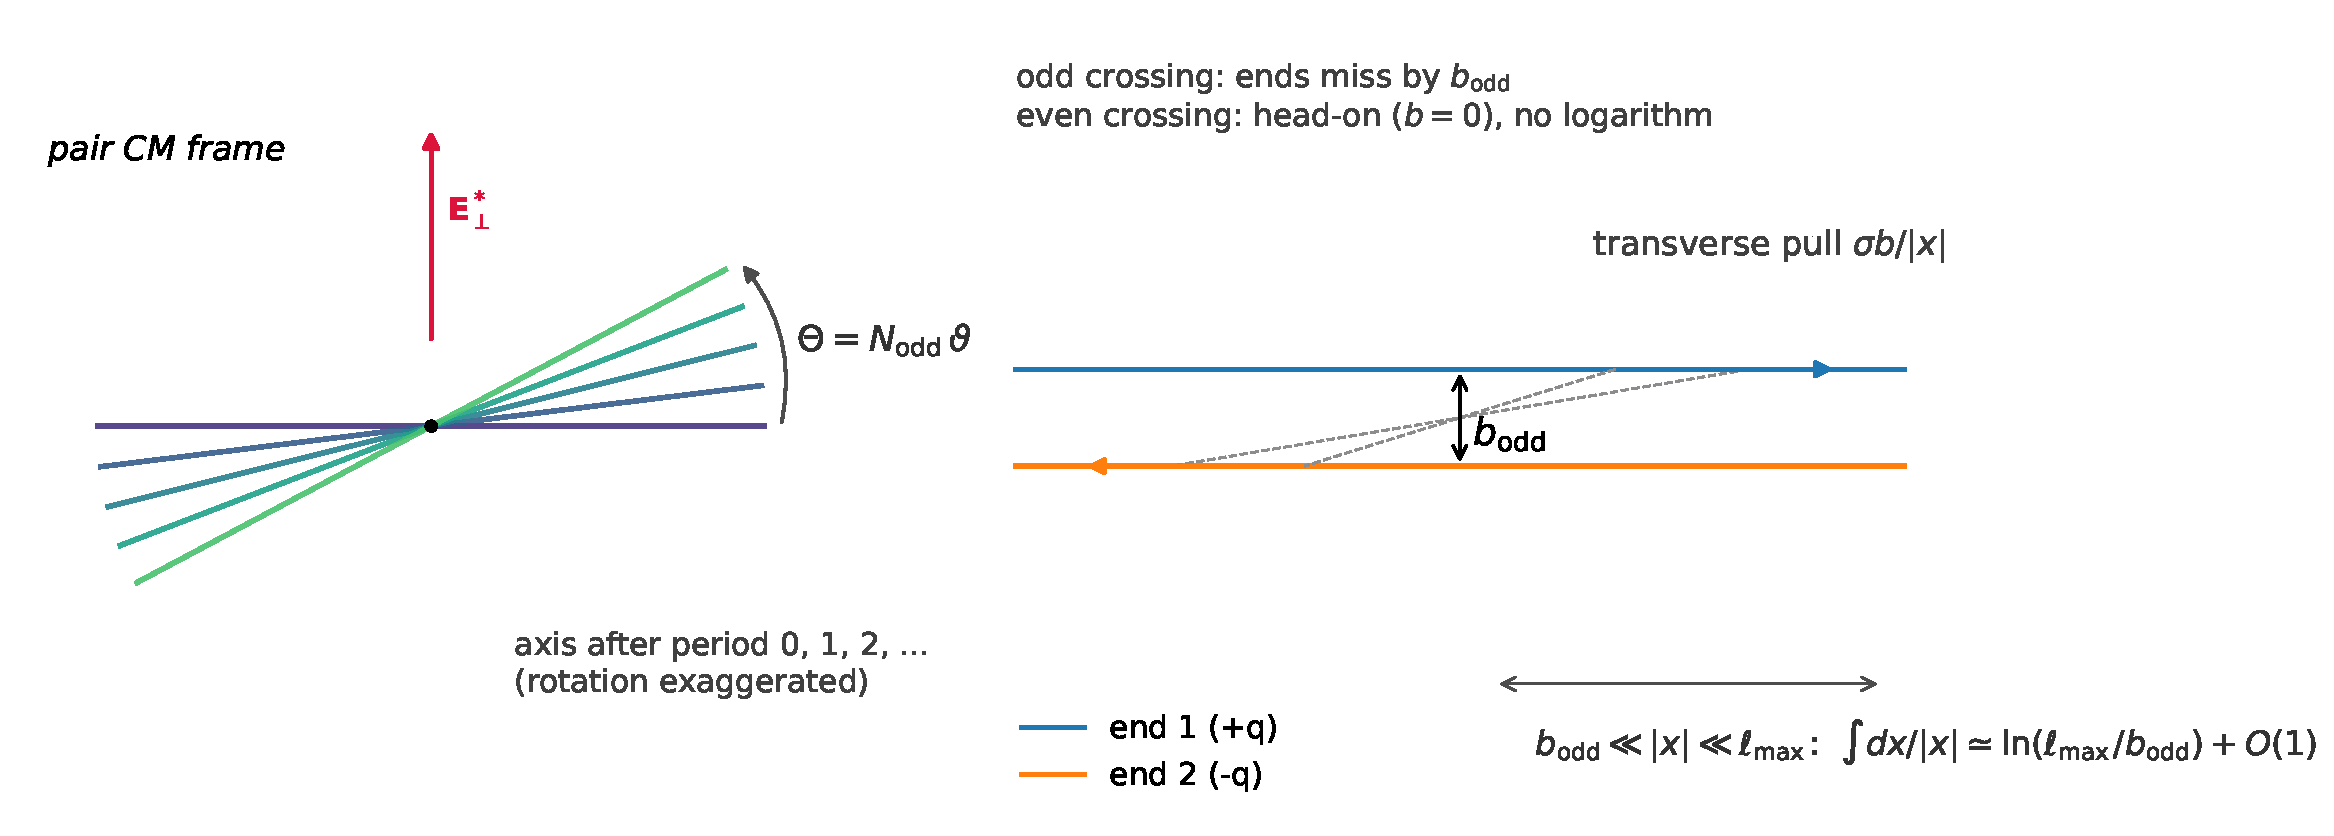
\includegraphics[width=0.92\linewidth,height=0.40\linewidth]{figures/schematic_nearmiss.pdf}
\caption{Schematic of the near-miss mechanism in the pair CM frame (conceptual diagram, not data; all scales
exaggerated). (Left) The oscillation axis turns by $\rot$ per period toward $\Estar_\perp$, coherently, so the rotation
accumulates as $\Theta=N_{\rm odd}\rot$. (Right) At an odd crossing the ends miss by $\bodd$, Eq.~\eqref{eq:bodd}; in
the region $\bodd\ll|x|\ll\lmax$ the string pulls the ends sideways with $\sigma\bodd/|x|$, whose integral gives the
logarithm of Eq.~\eqref{eq:rot}. Even crossings are head-on and carry no logarithm.}
\label{fig:schematic}
\end{figure}

\subsection{The per-period axis rotation}\label{sec:string:rot}
For a pure CM electric field ($\kB=0$) the rotation of the axis per CM period is
\begin{equation}
  \rot=\epsp\,G(\gst)\left[\ln\frac{\lmax}{\bodd}+K(\gst)\right],\qquad
  G(\gst)=\frac{2\left[\gst-\operatorname{asinh}(\gst\bst)/(\gst\bst)\right]}{\gst\bst\operatorname{artanh}\bst},
  \label{eq:rot}
\end{equation}
always toward $+\Estar_\perp$ and coherent from period to period, so that after $N_{\rm odd}$ odd crossings (one per period) the accumulated rotation is
$\Theta=N_{\rm odd}\rot$. The structure and $G$ are
derived; $G\to4/3$ in the non-relativistic limit, and $G=1.316/1.245/1.087/0.953$ at $\gst=1.05/1.28/2/3$. The slope of
$\rot/\epsp$ against $\ln(1/\epsp)$ in exact-NG numerics equals $G$ to 0.1--0.2\% at every $\gst$, which confirms the
retardation factor (the quasi-static $1/\bst$ would give slopes 1.03--1.87 times larger). The constant $K$ is analytic
only for slow ends, where a matched inner/outer calculation gives
\begin{equation}
  \rot_{\rm NR}=\tfrac43\,\epsp\left[\ln\frac{\lmax}{\bodd}+3\ln2-2\right],
  \label{eq:rotNR}
\end{equation}
i.e.\ $K(1)=3\ln2-2=0.0794$; at relativistic $\gst$ it is numerical (\EST{}, two solvers at $\gst=1.3$ and 2):
$K=+0.056/-0.049/-0.175/-0.309/-0.569$ at $\gst=1.05/1.28/1.6/2/3$, interpolated by
$K\simeq(3\ln2-2)-0.506\ln\gst-0.077\ln^2\gst$. Since $|K|\le0.6$ against $\ln(\lmax/\bodd)\approx8$--14, $K$ changes
the slope $c$ by at most 6\%.

\paragraph{Credit.} Li et al.\ observed that after each period the quirk system is rotated by a small angle (their
$\eta$), whose secular accumulation enters their thickness formula~\cite[Eqs.~(A.6), (A.17), (V.5)--(V.6),
(B.9)]{Li:2020aoq}; they determined it numerically and estimated $r|\eta|\sim d_E$. Equation~\eqref{eq:rot} is an
analytic expression for that angle. The logarithm itself is the elementary deflection of a nearly radial orbit passing a
constant-magnitude central force at impact parameter $b$; it is not a retardation or string-curvature effect, and a
step-converged straight-string integration has it too (Section~\ref{sec:string:valid}). Knapen et al.'s torque estimate
captures the scale $q|\Estar|/\sigma$ and the alternating half-period rotation~\cite[Eqs.~(8)--(9)]{Knapen:2017kly}, but
not the logarithmic secular term.

\subsection{The thickness law and the local slope $c$}\label{sec:string:law}
The plane fit sees only the component of the accumulated rotation out of the initial plane. Over the tracker the number
of periods scales as $\sigma$, the lever arm as $\lzero$, and $\rot\propto\epsp\propto qB/\sigma$, so the accumulated
tilt is $\sim qBR\,G[\ln(\lmax/\bodd)+K]/p^*$, a bending angle of momentum $p^*$ over $R$; the out-of-plane
displacement is this tilt times the lever arm $\sim\lzero\propto\mQ/\sigma$, i.e.\ $\propto qBR/\sigma=\epsB R$. With a
rotating-yo-yo model (the exact vacuum yo-yo whose axis steps by $\rot$ at each odd crossing, boosted to the lab; nothing
fitted) this gives
\begin{equation}
  \DsB=\frac{qBR}{\sigma}\,F\left[\ln\frac{1}{\epsB}+C\right],\qquad
  c\equiv\frac{d\ln(\DsB/\epsB)}{d\ln(1/B)}=\frac{1}{\ln(1/\epsB)+C},
  \label{eq:law}
\end{equation}
where $F$ is a dimensionless function of the CM velocities, angles and layer phases, independent of $\mQ$ and $\Lam$ at
fixed velocities, and $C=-\ln(\gamma_{\rm cm}\beta_{T,\rm cm}\sin\alpha)+\ln[(\gst-1)/(\gst-\operatorname{asinh}(\gst\bst)
/(\gst\bst))]+K(\gst)$ collects the event kinematics ($\alpha$ is the CM angle between $\Estar$ and $\hat n$). The model
population values are $C=0.43/1.23/1.62$ at $\mQ=200/500/1000\GeV$; Eq.~\eqref{eq:law} then predicts local exponents
\begin{equation}
  \frac{d\ln\DsB}{d\ln B}=1-c,\qquad \frac{d\ln\DsB}{d\ln\Lam}=-2+2c,\qquad \mathcal R(f)\equiv\frac{\DsB(fB)}{f\,\DsB(B)}=1+c\ln\frac1f .
  \label{eq:exponents}
\end{equation}
Limiting cases: for $B\to0$, $\DsB/B\propto\ln(1/B)$ (non-analytic); for $\alpha=0$ ($\Estar\parallel\hat n$) the
rotation vanishes. The model accuracy against the exact causal string, event by event, is 1--4\% (median) for
$\gst\lesssim1.6$, which covers 84--97\% of events at $500$--$1000\GeV$ and 66\% at $200\GeV$; it is 10--35\% off for
$\gst>2$ (16\% of events at $200\GeV$, 7\% at $500\GeV$), where the rotation is spread over the half period and the CM
magnetic field acts (\EST{}).

Table~\ref{tab:c} gives the predicted population medians of $c$. The predicted fall of $c$ with $\Lam$ (0.116 to 0.070
from 0.6 to $10\keV$ at $500\GeV$) is the main test of Eq.~\eqref{eq:law}. In terms of scaling, $\DsB\approx
\Lam^{-1.8}B^{0.9}$ and is flat in $\mQ$ within errors: the model medians are $33.5/31.1/29.5\um$ at
$200/500/1000\GeV$ and $1\keV$, because the $\mQ$ dependence of $C$ and of the $\gst$ spectrum compensate. The
$\mQ$-independent $B/\Lam^2$ scaling of the plane rotation was estimated by Knapen et
al.~\cite[Eqs.~(8)--(9)]{Knapen:2017kly}, and Li et al.\ found a mild $\mQ$ and $p_T$ dependence
numerically~\cite[Sec.~V, Fig.~4]{Li:2020aoq} (also Ref.~\cite[Fig.~4]{Li:2019wce}: the confinement-scale
dependence is much stronger than the mass dependence); what is new here is the logarithm, the exponents' departure from
$\Lam^{-2}B$, and the constants.\footnote{The form $\DsB\propto\epsB[1+c\ln(\Lam^2/qB)]$ with a constant $c$ is not
equivalent to Eq.~\eqref{eq:law}: it predicts a $B$ exponent of 0.944 instead of the measured 0.911.}

\begin{table}[htbp]
\centering
\caption{Predicted population median of the local slope $c$ of Eq.~\eqref{eq:law} (16--84\% range in parentheses),
rotating-yo-yo model on the project's truth-level event sample, $B_0=3.8112\tesla$, $|\eta_{\rm pair}|<1$ (Stage-1
note \S5.3, \rep{analytic/predictions.json}). The $1\keV$, $500\GeV$ entry is verified by blind numerics,
$0.105\pm0.002$ (Table~\ref{tab:numerics}).}
\label{tab:c}
\begin{tabular}{rcccccc}
\toprule
$\mQ$ [GeV] & $0.6\keV$ & $1\keV$ & $2\keV$ & $3\keV$ & $5\keV$ & $10\keV$\\
\midrule
200  & 0.128 & 0.113 (0.108--0.120) & 0.098 & 0.091 & 0.083 & 0.074\\
500  & 0.116 & \textbf{0.104} (0.098--0.112) & 0.091 & 0.085 & 0.078 & 0.070\\
1000 & 0.111 & 0.100 (0.095--0.107) & 0.088 & 0.082 & 0.076 & 0.068\\
\bottomrule
\end{tabular}
\end{table}

\subsection{Numerical verification}\label{sec:string:numerics}
The predictions were tested by an independent ``blind'' numerics campaign that did not see the analytic coefficients
before finishing (\rep{analytic/numerics/NUMERICS.md}). The production solver is a causal, piecewise-null NG string
(the construction of Artru and of the Lund model~\cite{Artru:1979ye,Andersson:1983ia}; for segmented strings see also
Ref.~\cite{Gubser:2016wno}), as implemented for quirks in the ATLAS Athena Geant4 extension (software path
\rep{Simulation/G4Extensions/Quirks}) by J.~Black and T.~Nelson and used by FASER~\cite[App.~A]{FASER:2026fsy}; the second solver is a
conformal-gauge delay ODE with a different formulation and arithmetic. Table~\ref{tab:numerics} compares the headline
numbers. Per crossing, the miss distance matches Eq.~\eqref{eq:bodd} to $10^{-4}$ in controlled CM-frame runs and to
0.6--2\% in full events; the per-crossing rotation matches the vacuum law to 1--2\%.

\begin{table}[htbp]
\centering
\small
\caption{Predictions of Section~\ref{sec:string} against blind numerics (truth level, field only, no material; Stage-1
note \S5.3, \S9; \rep{NUMERICS.md} \S0, \S4). $\mathcal R(f)$ is the response per unit field of Eq.~\eqref{eq:exponents} at
$\mQ=500\GeV$, $\Lam=1\keV$. ``Two solvers'' means causal and conformal codes agree.}
\label{tab:numerics}
\begin{tabularx}{\linewidth}{>{\raggedright\arraybackslash}Xccl}
\toprule
quantity & prediction & numerics & status\\
\midrule
$\bodd/(\epsp\lmax)$ at $\gst=1.05/1.3/2/3$ & 1.327/1.298/1.240/1.188 & 1.328/1.298/1.240/1.189 & two solvers\\
$c$ ($500\GeV$, $1\keV$) & 0.104 & $0.105\pm0.002$ & verified\\
$B$ exponent over $B_0/80\ldots B_0$ & 0.914 & $0.911\pm0.003$ & verified\\
$\mathcal R(1/2,1/4,1/20,1/80)$ & 1.072/1.144/1.311/1.455 & 1.073/1.147/1.320/1.460 & $\pm0.001$--0.005\\
$|q|=2$: $\DsB(2B_0)/\DsB(B_0)$ & $2[1-c\ln2]$ & ratio to pred.\ $0.999\pm0.001$ & verified\\
$K_{\rm vac}$ (non-relativistic) & $3\ln2-2=0.0794$ & $0.0791\pm0.0003$ & two solvers\\
\bottomrule
\end{tabularx}
\end{table}

\subsection{Validity, open terms and a failed prediction}\label{sec:string:valid}
\paragraph{The CM magnetic field.} In linear response $\Bstar$ neither changes $\bodd$ nor rotates the axis (its forces on
the two ends are odd under exchange), but it enters the non-linear inner region of the odd crossing. Measured in exact
NG runs, its effect on $\rot$ is even in $\Bstar$, vanishes for $\gst\to1$, is non-monotonic in $\kB$ and reaches
$-7$ to $-21\%$ at $\gst=2$ for $\kB=4$--16 (\EST{}; mechanism conjectural). Per event, $c$ shifts by $+17$ to $+36\%$
for $\kB=8$--12; events with $\kB>6$ are 5/29/43\% of the sample at $200/500/1000\GeV$, for which the per-event $c$ is
not reliable. \paragraph{Population-level status of $c$ (used throughout this note).} The prediction for the population median of
$c$ is confirmed by the blind numerics at $1\keV$ within $1.5\%$ ($0.105\pm0.002$ against 0.104,
Table~\ref{tab:numerics}). On the full-kinematics Stage-3 simulation (Section~\ref{sec:p1:law}) the per-event law
holds (paired agreement $\le1\%$ at $1\keV$), but the population median of the measured $c$ lies $+2$--$3\%$ above the
prediction at $1\keV$ ($+2.0/+2.1/+3.2\%$ at $E$ 500/$E$ 1500/$\Etil$ 500; $+0.7/+1.1\%$ at $E$ 200/1000), failing
the pre-set $1.5\%$ validation gate; pooled over $1$--$2\keV$ the excess is $+1.71\pm0.29\%$, which a zero-median
symmetric per-event scatter reproduces ($+2.04\%$), so we read it as an estimator effect (\EST{}). The population
uncertainty on $c$ at $1$--$2\keV$ is therefore quoted as $+2$--$3\%$; at $3$--$5\keV$ a larger, $\kB$-dependent excess
is attributed to $\Bstar$ (\EST{}, Section~\ref{sec:p1:law}).

\paragraph{Scale-free equivalence and the high-$\Lam$ systematic.} Scaling all coordinates by $\lambda$ maps a solution
for $(\sigma,qB)$ onto one for $(\sigma/\lambda,qB/\lambda)$: per oscillation $(\Lam\sqrt k,B)$ is the same physics as
$(\Lam,B/k)$, with $\Nosc$ larger by $k$. The law is verified at $\Lam\approx1\keV$ (blind numerics: population $c$ within
$1.5\%$, $C$ to 0.1--0.2; full simulation: $+2$--$3\%$, see above), consistent at $3$--$5\keV$ ($\lesssim1\%$ on $\DsB(5)/\DsB(3)$), and not verified above $\approx5\keV$, where
an excess seen in weak-field scans combines a cumulative $\Bstar$ part with a double-precision floor of both solvers
($\bodd/\lzero\approx3\times10^{-8}$). An unmeasured, unattributed systematic of order $\pm5\%$ on $\DsB$ (population;
sign expected positive) and up to tens of per cent on the per-event $c$ for $\kB\gtrsim10$ is therefore carried above
$5\keV$. Two decisive floor tests (extended precision on a scaled detector; reduced-precision emulation) are specified but
were not run.

\paragraph{Classical validity.} Classical NG holds at odd crossings while $\bodd\gg1/\Lam$, i.e.\ for $\Lam\lesssim10\keV$
for all events and up to $\Lam\approx26\keV$ for typical ones; beyond, the lower cut-off of the logarithm becomes $\sim1/\Lam$
and the model uncertainty on $\DsB$ is $\approx3$--8\% at $30\keV$ (\EST{}). Above $\Lcross\approx1.2$--$1.9\keV$ (depending on $\mQ$)
$\DsB$ is below the multiple-scattering floor anyway (Section~\ref{sec:p1:ms}).

\paragraph{Charge and spin.} Since $q$ enters only through $qB$, $\DsB(q)/\DsB(1)=q[1-\ln q/(\ln(1/\epsB)+C)]$, i.e.\
1.86 rather than 2 for $|q|=2$ (verified numerically, Table~\ref{tab:numerics}). This implies a $\approx c\ln2\approx7\%$
deviation from linearity in Li et al.'s factor-two charge test, consistent with their ``linearly proportional'' at their
precision~\cite[Sec.~V.A, Fig.~4]{Li:2020aoq}. Classical NG has no spin: for the scalar the per-event law is the same and
only the $\gst$ spectrum changes (median $\gst=1.39$ vs 1.23 at $500\GeV$), which roughly doubles the model uncertainty
(\EST{}).

\paragraph{Straight strings and a failed prediction.} Any attraction of fixed magnitude along the string gives
$\sigma b/|x|$ and hence the logarithm, so a step-converged straight-string (``Li-method'') integrator~\cite{Li:2019wce,Li:2020aoq}
also shows the $B\ln(1/B)$ response: its $c$ agrees with NG within $\approx3\%$ at $\gst=1.28$. The size of the
rotation differs, however, and the predicted straight-string/NG thickness ratio at $\gst=2$, 0.50, \textbf{fails}: the
measurement is $0.75\pm0.08$ (30 events; a 10-event subset at a finer step gives $0.96\pm0.10$), a $\approx3\sigma$
discrepancy. Three candidate causes ($\Bstar$ in the exact string, the breakdown of $\DsB\propto\rot$ at $\gst=2$, and a
frame-dependent miss-distance ratio) are identified but not quantified; the structural statements above are unaffected.
This answers the call for a direct check of the straight-string approximation~\cite[Sec.~3.2]{Kang:2008ea} and the
neglect of retardation in Ref.~\cite[Sec.~2]{Evans:2018jmd} at the level of a direct comparison, without implying an
error in published limits, which use the numerical thickness within an order of magnitude~\cite[App.~C]{Li:2020aoq}.

\paragraph{Scope.} By user decision, P1 is restricted to the B-field crossing physics: multiple scattering enters only as
the measured floor of Section~\ref{sec:p1}, with the Highland $\sqrt{x/X_0}$ scaling~\cite{Highland:1975pq,ParticleDataGroup:2024cfk}
credited, and no analytic multiple-scattering claim is made. Material-induced rotations of the quirk plane were estimated
and neglected by Knapen et al.~\cite[Sec.~II]{Knapen:2017kly} and studied for ionisation in the FASER geometry by Li et
al.~\cite[Sec.~4.1]{Li:2021tsy}. Classical strings with massive charged ends in constant fields were previously solved
only for motions linear in the endpoint proper time~\cite{Barbashov:1977tv}, which in 3+1 dimensions reduce to uniform
rotations~\cite{Petrov:1996wz}; the field-driven yo-yo with a near miss is outside that class.
